\chapter{Theoretical background}

The search presented in this thesis is for a simplified model of a supersymmetric theory. The amount of theoretical background required to fully understand  this theory can fill many books, and therefore, this document does not attempt to give an exhaustive description of it. Instead, I attempt to give a brief tour of topics that contribute to the understanding the subject, which are also of personal interest. Especially I wanted to also explore the theoretical motivation for supersymmetry, alongside a contribution to the philosophical discussion that normally accompanies such arguments. Whenever possible, I pick a description of a concept that I find intriguing and inspiring in a way that reminds me of my initial spark and inspiration for perusing a PhD in physics. Good sources for these topics are~\cite{Peskin2019-bt,Srednicki2007-mn}.

\section{Principle of Least Action}
\label{sec:least-action}
The earliest formulation of classical mechanics is normally attributed to the works of Sir Isaac Newton from the 17th century, which is also referred to as Newtonian mechanics. It is based on the then-newly developed mathematics of calculus. A central theorem in calculus is Fermat's theorem, which states that if a function has a local extremum at some point and is differentiable there, then the function's derivative at that point must be zero. The equation of motion is given by Newton's second law, which is an ordinary differential equation given by:

\begin{equation}
\vb{F}=\dv{\vb{p}}{t}=\dv{(m\vb{v})}{t}.
\label{eq:newton-second-law}
\end{equation}

When the mass $m$ is constant, this is equivalent to the famous $\vb{F}=m\vb{a}$. In modern physics, a more generalized approach is used based on an \emph{action}. It has been developed in the 18th centenary, and is able to reproduce Newtonian mechanics, but also able to generalize to handle Quantum Mechanics (QM), Relativistic Quantum Field Theory (RQFT) and even General Relativity (GR). The development of that principle was carried in different times by different people, and can be formulated in equivalent manners. In RQFT it is useful to use a \emph{Lagrangian} and therefore it will be shown here, rather than the \emph{Hamiltonian} formulation. The two formulations are equivalent, however. Given $N$ generalized coordinates $\vb{q}=\qty(q_1,q_2,\ldots,q_N)$, a \emph{Lagrangian} of the system is written $L\qty( \vb{q}\qty(t), \dot{\vb{q}}\qty(t), t )$. In non-relativistic mechanics for a system of particles in the absence of a magnetic field  $L=T-V$ where $T$ is the total kinetic energy of the system and $V$ is the potential energy of the system. For other systems, writing a Lagrangian is not straight forward, and we'll just assume that it is given. The \emph{action} of the system is a functional of the $N$ generalized coordinates, denoted $\mathcal{S}$, given by:
\begin{equation}
\mathcal{S}\qty[ \vb{q}, t_1, t_2 ] = \int^{t_2}_{t_1} L\qty( \vb{q}\qty(t), \dot{\vb{q}}\qty(t), t ) \dd t
\end{equation}
where the dot denotes the time derivative, and $t$ is time. The principle of least action is then:
\begin{quote}
The path taken by the system between times $t_1$ and $t_2$ and configurations $q_1$ and $q_2$ is the one for which the action is stationary (no change) to first order.
\end{quote}
Mathematically, that is equivalent to requiring $\delta \mathcal{S}=0$ or:
\begin{equation}
\delta \int^{t_2}_{t_1} L\qty( \vb{q}\qty(t), \dot{\vb{q}}\qty(t), t ) \dd t = 0.
\label{eq:principle-of-least-action}
\end{equation}

The principle of least action has been preceded by earlier ideas in optics, such as that for the path of light reflecting from a mirror, the angle of incidence equals the angle of reflection. The principle of least action is the variational equivalent in the calculus of variations of Fermat's theorem in calculus. It is used in order to find a path that extremizes the Lagrangian. Interestingly enough, Fermat also coined Fermat's principle, which states that "light travels between two given points along the path of shortest time", which is an earlier example of the principle of least action. Using this principle, one can arrive at the equations of motion of the system. For a classical system, those would be equivalent to  Newton's laws of motion Eq.~\ref{eq:newton-second-law}. Solving Eq.~\ref{eq:principle-of-least-action}, one arrives at Euler–Lagrange equations:
\begin{equation}
\pdv{L}{\vb{q}}-\dv{t}\pdv{L}{\vb{\dot{q}}}=0.
\end{equation}
Solving Euler–Lagrange equations gives the equations of motion of the system. In field theory, an analogous equation is used to calculate the dynamics of a field.

\section{The Quantum}
\label{sec:quantum}

The main object that is the subject of research in particle physics is, of course, a particle. More precisely, an elementary particle or fundamental particle, which is a subatomic particle that is not composed of other particles. The electron is an example of such a fundamental particle, which was also the first to be discovered by Thomson in 1897. The description and properties of the particles have radically evolved over time, and so did the mathematical language that is used to describe them. In classical electromagnetism for example, one can use abstractions such as a point charge, point mass or electron point by using a Dirac delta function $\delta$ in the charge and mass  distributions. In quantum mechanics, a wave function $\Psi(\vb{x},t)$,  that assigns a complex number to each point $\vb{x}$ at each time $t$, is used. The wave function is governed by the Schrödinger equation \cite{Liboff2002-vc,Cohen-Tannoudji1977-ms,Cohen-Tannoudji1977-rq}. The time-dependent Schrödinger equation is:
\begin{equation}
i\hbar\dv{t}\ket{\Psi(t)}=\hat{H}\ket{\Psi(t)}.
\label{eq:schrodinger-eq}
\end{equation}
For a single nonrelativistic particle in one dimension that becomes:
\begin{equation}
i\hbar\pdv{t}\Psi(x,t)=\qty[-\frac{\hbar^2}{2m}\pdv[2]{x}+V(x,t)] \Psi(x,t).
\label{eq:schrodinger-single-eq}
\end{equation}
The parameter $m$ is the mass of the particle, and $V(x,t)$ is the potential that represents the environment in which the particle exists. This can be easily generalized to include more than one particle. However, nonrelativistic quantum mechanics has a shortcoming, in that the Schrödinger equation for massive particles has a fixed number of particles governing the state of the system. It is not surprising given the fact that in classical mechanics, and therefore nonrelativistic quantum mechanics by extension, mass is never created nor destroyed. In order to accommodate the observation that particles are being created and destroyed, a relativistic treatment is needed. That is the goal of RQFT.

But the equivalent of particles DO actually arise in nonrelativistic quantum mechanics: when they are massless. In fact, the formalism for creating and destroying massless particles, quanta, is generalized from quantum mechanics to RQFT. The quantum arises in the quantum mechanical harmonic oscillator. Classically, a harmonic oscillator is a system that, when displaced from its equilibrium position, experiences a restoring force $F$ proportional to the displacement $x$:
\begin{equation}
\vb{F}=-k\vb{x},
\end{equation}
where $k$ is a positive constant. The potential energy stored in a simple harmonic oscillator at position $x$ is:
\begin{equation}
U=\frac{1}{2}kx^2.
\end{equation}
Writing a Hamiltonian and promoting the observables to operators we get:
\begin{equation}
\hat{H} = \frac{\hat{p}^2}{2m} + \frac{1}{2}k\hat{x}^2 = \frac{\hat{p}^2}{2m} + \frac{1}{2}m\omega^2 \hat{x}^2,
\end{equation}
where $m$ is the particle's mass, $k$ is the force constant, $\omega = \sqrt{k/m}$ is the angular frequency of the oscillator, $\hat{x}$ is the position operator, and $\hat{p}$ is the momentum operator. Solving the time-independent Schr{\"o}dinger equation gives the energy levels
\begin{equation}
E_n=\hbar\omega\qty(n+\frac{1}{2})=\qty(2n+1)\frac{\hbar}{2}\omega.
\end{equation}
It is interesting to note that the energies are quantized and equally spaced with discrete energy values of integer-plus-half multiples of $\hbar\omega$.

\subsection{Annihilation and Creation Operators}
\label{sec:ladder-operators}
We define ladder operators
\begin{equation}
\begin{split}
\hat{a} &\equiv \sqrt{\frac{m\omega}{2\hbar}} \left(  \hat{x} + \frac{i\hat{p}}{m\omega_0}  \right) \\
\hat{a}^\dagger &\equiv \sqrt{\frac{m\omega}{2\hbar}}\left(  \hat{x} - \frac{i\hat{p}}{m\omega_0}  \right).
\end{split}\label{ac}
\end{equation}
As can be seen, $\hat{a}$ is not Hermitian. 
Using $\left[ \hat{x}, \hat{p}  \right] = i\hbar$ it is easy to show that
\begin{equation}\label{acom}
\begin{split}
&\left[ \hat{a}, \hat{a}^\dagger  \right] = 1\\
&\hat{a} \hat{a}^\dagger = 1 + \hat{a}^\dagger  \hat{a}.
\end{split}
\end{equation}
By reversing \ref{ac} we get
\begin{equation}\label{xho}
\hat{x} = \sqrt{\frac{\hbar}{2m\omega}}\qty(\hat{a} + \hat{a}^\dagger)\, ,\qquad
\hat{p} = i\sqrt{\frac{\hbar m \omega}{2}} \qty(\hat{a} - \hat{a}^\dagger)
\end{equation}
and the Hemiltonian becomes
\begin{equation}
\hat{H} = \hbar\omega_0\left(  \hat{a}^\dagger  \hat{a}+ \frac{1}{2} \right) \equiv \hbar\omega_0\left( \hat{N} + \frac{1}{2} \right).
\end{equation}
Finding eigenvalues for $\hat{H}$ becomes finding eigenvalues of the \emph{number operator} $\hat{N} \equiv  \hat{a}^\dagger  \hat{a}$, which are
\begin{equation}
N\ket{n}=n\ket{n}.
\end{equation}
Operating with the ladder operators on the energy eigenstates gives
\begin{equation}
\begin{split}
\hat{a}^\dagger \ket{n} &= \sqrt{n+1}\ket{n+1}\\
\hat{a}\ket{n} &= \sqrt{n}\ket{n-1}.
\end{split}
\end{equation}
It is seen that $\hat{a}^\dagger$, in essence, appends a single quantum of energy to the oscillator, while $\hat{a}$ removes a quantum. Furthermore, acting with the number operator $\hat{N}$ yields
\begin{equation}
\begin{split}
N\hat{a}^\dagger \ket{n} &= (n+1)\hat{a}^\dagger\ket{n} \\
N\hat{a}\ket{n} &= (n-1)\hat{a}\ket{n}.
\end{split}
\end{equation}
Due to this, $\hat{a}$ is called a annihilation operator ("lowering operator"), and $\hat{a}^\dagger$ a creation operator ("raising operator"). The two operators together are called ladder operators. In quantum field theory, these operators destroy and create particles, which correspond here to a quanta of energy of $\hbar\omega$.

\section{Relativistic Quantum Field Theory}

In the first quarter of the twentieth century, two of the most successful theories in modern physics have been developed, special relativity and quantum mechanics. Special relativity was necessary to solve the incompatibility of Maxwell's equations of electromagnetism with Newtonian mechanics. In addition, experimentally,  the Michelson–Morley experiment's null result demonstrated that the historically hypothesized luminiferous aether did not exist. Special relativity diverges from classical mechanics in high-velocities. Quantum mechanics, on the other hand, arose gradually from theories to explain observations that could not be reconciled with classical physics, such as Max Planck's solution to the black-body radiation problem, and the correspondence between energy and frequency in Albert Einstein's photoelectric effect. Quantum mechanics differs from classical physics in that energy, momentum, angular momentum, and other quantities of a bound system are restricted to discrete values; objects have characteristics of both particles and waves; and there are limits to how accurately the value of a physical quantity can be predicted prior to its measurement, given a complete set of initial conditions (the uncertainty principle).

Since classical mechanics diverged into two different directions, namely, quantum mechanics and special relativity (which later on developed further into general relativity, but that's beyond the concern here), it was clear that a theory that incorporates both developments is needed. The first effort came from an attempt in creating a quantum mechanical theory of the electromagnetic field. It was also crucial to develop a theory, in which the number of particles changes, in order describe processes such as a $\beta$-decay or the emission of a photon by an electron dropping into a quantum state of lower energy in an atom.

Quantum field theory successfully combines classical field theory, special relativity, and quantum mechanics. QFT treats particles as excited states (also called quanta) of their underlying quantum fields, which are more fundamental than the particles. The equation of motion of the particle is determined by minimization of the Lagrangian, a functional of fields associated with the particle. Interactions between particles are described by interaction terms in the Lagrangian involving their corresponding quantum fields. Each interaction can be visually represented by Feynman diagrams according to perturbation theory in quantum mechanics.

\subsection{Attempts at Relativistic Quantum Mechanics}
\label{sec:attempts-rqt}

At first glance, fields are not the only way to try and reconcile quantum mechanics and relativity. A naive attempt~\cite{Srednicki2007-mn} could be to take the Schrödinger equation~\ref{eq:schrodinger-eq} and write a Hamiltonian in a relativistic notion $H=\sqrt{\hat{\vb{p}}^2+m^2}$ (taking as usual $\hbar=c=1$). Plugging it as is into the Schrödinger equation will result in the time derivative outside the square root, while the space derivatives under it, which is not in the spirits of relativity. Squaring the differential operators before applying them to the wave function and collecting terms results in the \emph{Klein-Gordon equation}:
\begin{equation}
\qty(\pdv[2]{t}-\nabla^2+m^2)\Psi\qty(\vb{x},t)=0.
\label{eq:kg-wf}
\end{equation}
It is second-order in both space and time derivatives, and they appear in a symmetric fashion. The $\Psi$ in the equation is the usual quantum mechanical wave function. There are two problems with sticking to the wave function. The first, is that the norm of a state $\braket{\Psi,t}$ is not in general time independent. Thus probability is not conserved. The Klein-Gordon equation obeys relativity, but not quantum mechanics. This specific problem is solved (for spin-one-half particles) by the \emph{Dirac equation}. In its original form written by Dirac~\cite{Dirac1981-rt}:
\begin{equation}
\qty(\beta m c^2 + c\sum^3_{n=1}\alpha_n p_n)\Psi\qty(\vb{x},t)=i\hbar\pdv{\Psi\qty(\vb{x},t)}{t}
\label{eq:dirac-wf}
\end{equation}
where $\Psi\qty(\vb{x},t)$ again is to interpreted as an ordinary quantum mechanical wave function for the electron of rest mass $m$ with spacetime coordinates $x, t$. The $p_1,p_2,p_3$ are the components of the momentum, understood to be the momentum operator in the Schrödinger equation. The new elements in this equation are the four $4\times 4$ matrices $\alpha_1,\alpha_2\alpha_3$ and $\beta$, and the four-component wave function $\Psi$. There are four components in $\Psi$ because the evaluation of it at any given point in configuration space is a bispinor. It is interpreted as a superposition of a spin-up electron, a spin-down electron, a spin-up positron, and a spin-down positron. The $4\times 4$ matrices $\alpha_k$ and $\beta$ are all Hermitian and satisfy:
\begin{equation}
\alpha_i^2=\beta^2=I_4,
\end{equation}
and they all mutually anticommute:
\begin{equation}
\begin{split}
&\alpha_i \alpha_j + \alpha_j \alpha_i = 0 \:(i\neq j) \\
&\alpha_i \beta + \beta \alpha_i = 0.
\end{split}
\end{equation}
It turns out that the Dirac equation is fully consistent with relativity provided. There are, however, some problems. The minimum size of the matrices of $4\times 4$ imply extra two "spin" states. They also imply negative eigenvalues for the Hamiltonian which indicate that there is no ground state. Dirac postulated his famous \emph{Dirac sea} of electrons to suggest that the negative energy states are all occupied. An electron in the sea could then be excited to a positive energy state leaving behind a \emph{hole} in the Dirac sea. This hole would appear to have positive charge, and positive energy. Dirac therefore predicted (in 1927) the existence of the positron, a particle with the same mass as the electron, but opposite charge. The positron was found experimentally five years later.

The problem with this solution though, is that we've started by trying to describe a theory of a single half-spin particle, and ended up describing a theory with infinite amount of particles. Even if this is taken to be satisfactory, this theory still cannot describe particles that do not obey Pauli exclusion, such as photons or pions. The problem lies in the difference between the way that nonrelativistic quantum mechanics and special relativity treats space and time. In special relativity, space and time are treated on equal footing. In nonrelativistic quantum mechanics, however, space is an operator, while time isn't. It turns out that turning time into an operator is a very difficult problem. The approach that proved to be fruitful is to make space a \emph{label}, just as time is, by turning the wave function $\Psi$ into a \emph{field}. Space and time are now labels in a \emph{quantum field} $\varphi(\vb{x},t)$ of operators. Each point in space and time now point to an operator. This allows one to really treat space and time on an equal footing.

\subsection{Classical Field Theory}
\label{sec:classical-field}

After the naive attempts at a relativistic quantum mechanics introduced in Section~\ref{sec:attempts-rqt}, two successful and widely used methods of constructing quantum field theories are described in Section~\ref{sec:quantization}. The first is the canonical quantization in Section~\ref{sec:canonical}, and the second is the path integrals formalism in Section~\ref{sec:path-integrals}. They involve starting from a classical field theory and quantizing it. In a classical field theory, the equation of motion can be derived from variation of an action $\mathcal{S}=\int \dd{t}L$, where $L$ is the Lagrangian, which is the spatial integral of a Lagrangian density $\mathcal{L}$, so that $L=\int \dd[3]x\mathcal{L}$. The Lagrangian density is a function of one or more fields $\phi(x)$, and their derivatives $\partial_{\mu}\phi$, so that
\begin{equation}
\mathcal{S}=\int \dd{t}L=\int \mathcal{L}\qty(\phi,\partial_{\mu}\phi)\dd[4]x.
\end{equation}
Following the principle of least action described in Section~\ref{sec:least-action}, we we take the action $\mathcal{S}$ to an extremum and write
\begin{equation}
\begin{split}
0 & =  \delta \mathcal{S} \\
& = \int \mathrm{d}^4 x \left\lbrace \frac{\partial\mathcal{L}}{\partial\phi}\delta\phi + \frac{\partial\mathcal{L}}{\partial\left(\partial_\mu\phi\right)}\delta\left(\partial_\mu\phi\right) \right\rbrace \\
& = \int \mathrm{d}^4 x \left\lbrace \frac{\partial\mathcal{L}}{\partial\phi}\delta\phi - \partial_\mu \left(   \frac{\partial\mathcal{L}}{\partial\left(\partial_\mu\phi\right)} \right) \delta\phi   +   \partial_\mu \left(   \frac{\partial\mathcal{L}}{\partial\left(\partial_\mu\phi\right)}  \delta\phi \right) \right\rbrace .
\end{split}
\end{equation}
The last term can be turned into a surface integral over the boundary of the region of integration. Since $\delta\phi$ vanish on the spatial boundary, then the surface term is zero. After rearrangement, we arrive at the Euler-Lagrange equation of motion for a field,  
\begin{equation}
\partial_\mu \left(   \frac{\partial\mathcal{L}}{\partial\left(\partial_\mu\phi\right)} \right) - \frac{\partial\mathcal{L}}{\partial\phi} = 0 .
\end{equation}
If the Lagrangian contains more than one field, there is one such equation for each. The Hamiltonian of a discrete system can be written as
\begin{equation}
H \equiv \sum p\dot{q} - L,
\end{equation}
where $q$ is a dynamical variable, and $p\equiv \pdv*{L}{\dot{q}}$ is the conjugate momentum. To generalize to continuous system we define the \emph{momentum density} conjugate to $\phi\qty(\vb{x})$ as
\begin{equation}
\pi\qty(\vb{x})\equiv\pdv{\mathcal{L}}{\dot{\phi}\qty(\vb{x})},
\end{equation}
and the Hamiltonian can be expressed, using the Hamiltonian desnsity $\mathcal{H}$ as:
\begin{equation}
H = \int \mathrm{d}^3x [\pi(\mathbf{x})\dot{\phi}(\mathbf{x}) - \mathcal{L}] \equiv \int \mathrm{d}^3x \mathcal{H} .
\end{equation}
As an example, consider the theory of a single real scalar field $\phi\qty(x)$ with the Lagrangian
\begin{equation}
\mathcal{L} = \frac{1}{2}\left( \partial_\mu \phi \right)^2-\frac{1}{2}m^2\phi^2.
\label{eq:kg-lagrangian}
\end{equation}
Following the usual procedure and applying the Euler-Lagrange equation gives the equation of motion
\begin{equation}
\left(\partial^\mu\partial_\mu + m^2\right)\phi=0,
\end{equation}
which is the well-known Klein-Gordon equation. Here, $\phi$ is a classical field, and not a wave function, nor a quantum field. The Hamiltonian that results from the procedure described above is
\begin{equation}
H = \int \mathrm{d}^3x\left[ \frac{1}{2}\pi^2 + \frac{1}{2}\left( \nabla\phi \right)^2 + \frac{1}{2}m^2\phi^2  \right].
\end{equation}

\subsection{Quantization}
\label{sec:quantization}

As described in Section~\ref{sec:classical-field}, two methods of constructing quantum field theories are widely used. The first is the canonical quantization in Section~\ref{sec:canonical}, and the second is the path integrals formalism in Section~\ref{sec:path-integrals}. The path integrals formalism has an advantage in that it uses the Lagrangian formalism rather than the Hamiltonian. The Lagrangian formalism is explicitly Lorentz invariant, and in general, it is in practice easier to guess the correct form of the Lagrangian of a theory, which naturally enters the path integrals than the Hamiltonian. The advantage of the canonical quantization is that unitarity of the S-matrix is more explicit than in the path integral approach. The methods are described here in a very qualitatively manner. For an explicit mathematical formulation, Ref.~\cite{Peskin2019-bt,Srednicki2007-mn} are great sources for that.

\subsubsection{Canonical Quantization}
\label{sec:canonical}

Canonical quantization starts with a classical field theory, and then \emph{quantized} by promoting the dynamical variables to operators that obey canonical commutation relations. It can be demonstrated with the example of the Klein-Gordon case, which has the classical Lagrangian~\ref{eq:kg-lagrangian}. Promoting the field and momentum density to operators, the commutation relations generalize to:
\begin{equation}
\begin{split}
\comm{\phi\qty(\vb{x})}{\pi\qty(\vb{y})}&=i\delta^{(3)}\qty(\vb{x}-\vb{y});\\
\comm{\phi\qty(\vb{x})}{\phi\qty(\vb{y})}&=\comm{\pi\qty(\vb{x})}{\pi\qty(\vb{y})}=0.
\end{split}
\end{equation}
Writing the Klein-Gordon equation in Fourier space, one gets:
\begin{equation}
\qty[\pdv[2]{t} + \qty(\abs{\vb{p}}^2+m^2)]\phi(\vb{p},t)=0.
\end{equation}
This is the same as the equation of motion for a simple harmonic oscillator with the frequency $\omega_{\vb{p}}=\sqrt{\abs{\vb{p}^2+m^2}}$. Therefore a similar treatment to Section~\ref{sec:quantum} can be done here. Ladders operators are introduced, only that now each Fourier mode of the field is treated an an independant oscillator with it own $a$ and $a^\dagger$. The spectrum of the Klein-Gordon Hamiltonian can then be found in the same manner, and can be written as:
\begin{equation}
H=\int \frac{\dd^2 p}{(2\pi)^3} \omega_{\vb{p}}\qty(a^\dagger_{\vb{p}}a_{\vb{p}}+\frac{1}{2}\comm{a_{\vb{p}}}{a^\dagger_{\vb{p}}}).
\end{equation}
The operator $a^\dagger_{\vb{p}}$ created a particle with momentum $\vb{p}$ and energy $\omega_{\vb{p}}=\sqrt{\abs{\vb{p}^2+m^2}}$. The particles follow the proper relativistic energy-momentum relation, and have strictly positive energy. Since $a^\dagger_{\vb{p}}$ and $a^\dagger_{\vb{q}}$ commute, two particles are interchangeable. Moreover, since arbitrarily many particles can be produced for a single mode $\vb{p}$, the particles obey \emph{Bose-Einstein statistics}. In a theory of half-integer spin particles, anticommutators are to be used. The next steps in this formalism is to compute correlation functions, and eventually write down the full Feynman rules for the theory, in order to compute cross sections and decay rates.

\subsubsection{Path Integrals}
\label{sec:path-integrals}

The path integral formalism is an alternative construction to quantum mechanics developed by Richard Feynman, and is proven to be equivalent to the wave equation of Schrödinger, and the matrix algebra of Heisenberg, Born and Jordan. It is also used as an alternative way to construct quantum field theories, as an alternative to the canonical quantization. Using this formalism, it is easier compute propagators and derive Feynman rules. It also generalize better to non-Abelian gauge theories. Moreover, since it uses the Lagrangian, rather than the Hamiltonian, as its fundamental quantity, it explicitly preserves all symmetries of a theory. Using path integrals allows the direct computation of the scattering amplitude of a certain interaction process, rather than the establishment of operators and state spaces. 

Suppose we are interested to compute the amplitude for a particle to travel from one point $x_a$ to another $x_b$ in a given time $T$. The amplitude $U\qty(x_a,x_b,T)$ in the canonical Hamiltonian formalism using the time evolution operator is given by
\begin{equation}
U\qty(x_a,x_b,T)=\mel{x_b}{e^{-iHT/\hbar}}{x_a}
\end{equation}.
In the path integral approach, the total time T is divided into N small intervals, and the overall amplitude is the product of the amplitude of evolution within each interval, integrated over all intermediate states. The propagation amplitude becomes
\begin{equation}
\mel{x_b}{e^{-iHT/\hbar}}{x_a}=U\qty(x_a,x_b,T)=\int \mathcal{D}x(t)e^{iS\qty[x(t)]/\hbar},
\end{equation}
where $S\qty[x(t)]$ is the classical action, and $\int \mathcal{D}x(t)$ is another way of writing "sum over all paths". The functional formula then allows for the calculation of correlation functions, and eventually write down the full Feynman rules for the theory.

\subsection{Interactions}

The goal of every scientific theory is to make predictions about measurements. In the context of quantum field theory, it is normally one of two generic cases: one incoming particle, for which a decay rate is computed, or two incoming particles, for which a cross section is computed. For this, a recipe for computing a scattering amplitude and converting it into a measurable is needed.

\subsubsection{The Cross Section and Decay Rate}

The \emph{cross section} is the likelihood of any particular final state from collusion of two beams of particles with well-defined momenta. The \emph{cross section}, which has the units of area, denoted by $\sigma$ is the total number of events (of whatever type desired) divided by all of the quantities:
\begin{equation}
\sigma \equiv \frac{\text{Number of scattering events}}{\rho_\mathcal{A}\,l_\mathcal{A}\,\rho_\mathcal{B}\,l_\mathcal{B}\,A}
\end{equation}
where $\mathcal{A}$ are particles at rest with density $\rho_\mathcal{A}$, aimed by particles of type $\mathcal{B}$ with density $\rho_\mathcal{B}$ with velocity $v$, and $l_\mathcal{A}$ and $l_\mathcal{B}$ are the lengths of the bunches of particles. $A$ is the cross-sectional area common to the two bunches. We get
\begin{equation}
\text{Number of events} = \sigma\,l_\mathcal{A}\,l_\mathcal{B}\int d^2 x\,\, \rho_\mathcal{A}(x)\,\rho_\mathcal{B}(x)
\end{equation}
The \emph{differential cross section} is $d\sigma/(d^3 p_1\ldots d^3p_n)$ which when integrated over any small $d^3 p_1\ldots d^3p_n$ gives the cross section for scattering into that region of final-state momentum space. Cross sections are computed for a production of a specific process. The \emph{decay rate} $\Gamma$ of an unstable particle $\mathcal{A}$ assumed to be at rest into a specified final state is defined as
\begin{equation}
\Gamma \equiv \frac{\text{Number of decays per unit time}}{\text{Number of $\mathcal{A}$ particles present}}.
\end{equation}

\subsubsection{Interacting Fields}

The example that was used in previous sections, the Klein-Gordon field, was a free field theory. No interactions and no scattering were involved. In reality, particles do interact and scatter of each other. In order to obtain such interactions, nonlinear terms must added to the Lagrangian. One example of such interacting Lagrangian is the "phi-fourth" theory,
\begin{equation}
\mathcal{L} = \frac{1}{2}(\partial_\mu\phi)^2-\frac{1}{2}m^2\phi^2 -\frac{\lambda}{4!}\phi^4
\end{equation}
where $\lambda$ is a dimensionless \emph{coupling constant}. The goal is to be able to compute scattering amplitude for an interacting theory, in order to convert them into cross sections. This is generally impossible to solve exactly. Instead it is computed in the framework of \emph{perturbation theory}. It turns out that the perturbation series is quite simple in structure, and can be visualized with the use of \emph{Feynman diagrams}.

\subsection{Feynman Diagrams}

In order to compute cross sections and decay rates, one must compute matrix elements of the S-matrix. The S-matrix gives the probability amplitude for a scattering event between \emph{in} and \emph{out} states. The probability amplitude for producing the final state is simply related to the cross section. Computing the S-matrix elements, or scattering amplitudes, is done differently depending on the quantization scheme, canonical or path integrals. As previously mentioned, the computation is done in a perturbation series. A Feynman diagram is a graphical representation of a perturbative contribution to the transition amplitude or correlation function. In the canonical quantization, a Feynman diagram represents a term in the Wick's expansion of the perturbative S-matrix. 

The quantization scheme also provide \emph{Feynman rules} in order to compute the value of each Feynman diagram. It involves providing a mathematical expression for a \emph{propagator} for each internal line, or a virtual particle. Each diagram then has an amplitude which is a term in the perturbative expension. In Figure~\ref{fig:e-to-mu-feynman}, an example of a tree-level diagram representing a process of $e^+ e^- \rightarrow \mu^+ \mu^-$ through a photon $\gamma$ is shown.

\begin{figure}[!htb]
\centering
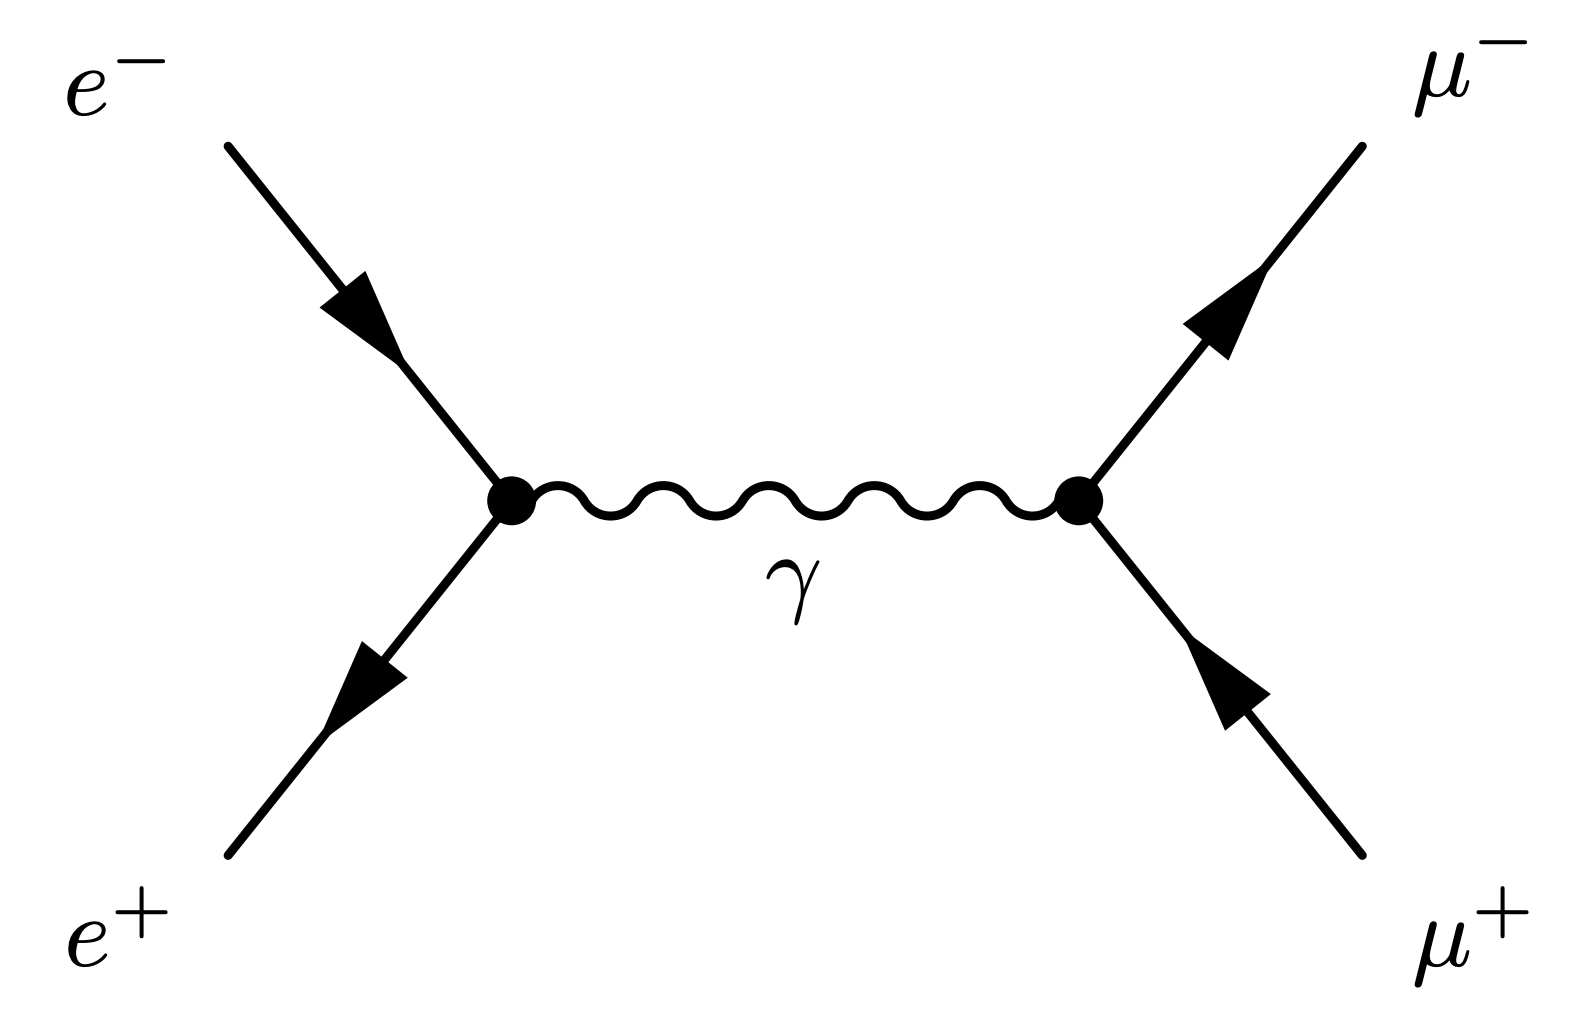
\includegraphics[width=0.5\linewidth]{plots/feynman_diagrams/feynman_e_to_mu.png}  \\
\caption[Electrons to Muons Feynman diagram]{Feynman diagram representing the tree-level process of $e^+ e^- \rightarrow \mu^+ \mu^-$. Electron and positron annihilate each other and produce muon-antimuon pair through a virtual photon.}
\label{fig:e-to-mu-feynman}
\end{figure}

\subsection{Renormalization}

\clearpage
\section{Symmetries}

In 1964, Richard Feynman gave a series of seven lectures called \emph{The Character of Physical Law} at Cornell University, as part of the Messenger Lectures series. The lectures were videotaped by the BBC, and are available online alongside their transcripts~\cite{Feynman1997-vo}. It is such a precious piece of history, and I would recommend everyone to watch it, as it is meant for the public audience. It showcases not only Feynman's ability to explain complex ideas and theories, but also his funny and enchanting personality. The fourth lecture in that series is called \emph{Symmetry in Physical Law}, in which he starts by describing how Weyl defines a symmetry:

\begin{quote}
So, Weyl said, a thing is symmetrical if there’s something that you can do to it, so that after you’re finished doing it, it looks the same as it did before. That is the sense in which we say that the laws of physics are symmetrical: that there are things that we can do to the physical laws, or to our way of representing the physical laws, which make no difference and leave everything unchanged in its effects.
\end{quote}

Most physicists will probably agree that that's what they mean when they say that a physical law is symmetrical. In this chapter we are concerned with symmetries of laws, rather then symmetries of objects, such as a human face, for example. In modern physics, hugely thanks to Noether's theorem, symmetries became fundamental, and they set the foundations of the Standard Model of particle physics. In this chapter I summarize the reasons why symmetries are so important, and what roles they play in the Standard Model. But first, I would like to introduce my favorite physics riddle, which Feynman described, starting at minute 40:04 in the same lecture:

\begin{quote}
Suppose that we were in telephone conversation with a Martian or an Arcturian, or something. We don’t know where he is and we would like to describe things to him. We want to tell him about things. You say, so how’s he going to understand the words, well, that’s been studied very much by Professor Morrison here. He has pointed out that one way would be to start out and say tick tick two, tick tick tick three, and so on, and pretty soon the guy’d catch onto the numbers. Then—as he understands your number system, then—you can write lots of numbers and you could, for example, write a whole sequence of numbers that represents the weights, the proportional weights, of the different atoms, in succession.

Then say, hydrogen: 1.008, deuterium, and so on and so on. And he would-after he sat down with all those numbers and piddled around a while, would-discover that the mathematical ratios were the same as the ratios of the weights of the elements and, therefore, those names must be for the elements—and so gradually, you could, in talking to him, have a common language, in many ways, common. There are many-now comes the problem.

Suppose that he says, you fellas—after we get familiar with him, he says, "You’re very nice; now I’d like to know what you look like." And you start out, "Well, we’re about six feet tall." He says, "Six feet, how big is a foot?" "It’s very easy," you say; "six feet tall is 170 thousand million hydrogen atoms high." Well, it’s not a joke; it’s a possible way of describing six feet to someone that has no measure, assuming that we cannot send him any samples, nor can we both look at the same object.

If we have to tell him how big we are; we can do it. That’s because the laws of physics are not unchanged under a scale change. We can use that factor, use the properties of the scale to determine—I mean, you can use that fact to determine the scale.

Well, here we’ve described ourselves after telling six feet tall, and we’re so-and-so bilateral on the outside, and we look like this, and there are these prongs sticking out, and all this. And he says, "That’s very interesting; what do you look like on the inside?" So we describe the heart and so on, and we say, "Now, put the heart in on the left side."

Now the question is, how can we tell him which side is the left side?
\end{quote}

Putting it short, the riddle is how to communicate the concept of left and right via radio signals to an alien civilization without reference to common sightings? Most physicists attempt this problem by thinking of the right-hand rule in electromagnetism. Unfortunately, that would not work. The correct solution is very unexpected, and one of the most surprising results of modern physics. The solution is explain in the section about parity symmetry~\ref{sec:parity}.

\subsection{Conservation Laws}

A conservation law states that a particular measurable property of an isolated physical system does not change as the system evolves over time. Conservation laws are useful because they describe which processes can or cannot occur in nature. They also allow properties of the motion to be derived without solving the equations of motion. Conservation laws have changed throughout history, and some are a part of one theory but not another. Mass, for example, is conserved in classical mechanics, but not in relativity due to the principle of mass–energy equivalence. However, it a good approximation when the assumptions of classical mechanics hold, such as low velocities and energies, and large enough objects. Most conservation laws are exact, or absolute, in the sense that they apply to all possible processes. Some conservation laws are partial, in that they hold for some processes but not for others.

In continuum mechanics, the most general form of an exact conservation law is given by a continuity equation. For example, conservation of electric charge $q$ is
\begin{equation}
\pdv{\rho}{t}=-\nabla\cdot\vb{j},
\end{equation}
where $\rho$ is the density of $q$ (amount per unit volume), $\vb{j}$ is the flux of $q$ (amount crossing a unit area in unit time), and $t$ is time. There are several methods for identifying conservation laws. It can be hypothesize and proved mathematically. In classical mechanics, Hamilton–Jacobi equations provide a method for identifying constants of motion, and so does Poisson's theorem. In quantum mechanics, an observable quantity $Q$ will be a constant of motion if it commutes with the hamiltonian, and it does not itself depend explicitly on time. In the context of particle physics, the most powerful theorem invoked in order to study conservation laws is Noether's theorem~\ref{sec:noethers-theorem}. It also this  theorem that connects conservation laws to symmetries, which is the topic of this section. 

Currently, exact conservation laws that have never been proven to be violated include conservation of mass-energy $E$, conservation of linear momentum $\vb{p}$, conservation of angular momentum $\vb{L}$, conservation of electric charge, conservation of weak isospin, conservation of color charge, conservation of boost 3-vector, and conservation of CPT parity. Approximate conservation laws, \ie, conservation laws which are approximately true in particular situations, such as low speeds, short time scales, or certain interactions include conservation of mechanical energy, mass, baryon number, lepton number, flavor, strangeness, space-parity, charge-parity, time-parity, and CP parity.

\subsection{Noether's Theorem}
\label{sec:noethers-theorem}

In 1915, German-Jewish female mathematician Amalie Emmy Noether proved one of the most fundamental theorems of 20th century's modern physics. In spring of that year, she was invited by David Hilbert and Felix Klein to join the Göttingen mathematics department, challenging the views of some of his colleagues that a woman should not be allowed to teach at a university. Soon after arriving at Göttingen, she demonstrated her capabilities by proving the theorem now known as Noether's theorem, which shows that a conservation law is associated with any differentiable symmetry of a physical system~\cite{Lederman2004-fl}. That made modern theoretical physicists much more focused on symmetries.

Informally, Noether's theorem can be stated as:
\begin{quote}
If a system has a continuous symmetry property, then there are corresponding quantities whose values are conserved in time.
\end{quote}
In the context of classical field theory, it can be stated as:
\begin{quote}
To each differentiable symmetry of a local Lagrangian, there corresponds a conserved current.
\end{quote}
Previously, we described a symmetry by something that you can do, so that it looks the same as it did before. More formally in this context, a symmetry is the covariance of the form that a physical law takes, where by covariance, we mean invariance of the form of physical laws under differentiable transformations. That means, continuous transformation that leave the equations of motion invariant invariant. Formally, in the context of classical field theories, the theorem can be stated in the language of fields~\cite{Peskin2019-bt}. Consider a continuous transformations on the fields $\phi$, which in infinitesimal form can be written
\begin{equation}
\phi(x)\rightarrow\phi^\prime(x)=\phi(x)+\alpha\Delta\phi(x),
\label{eq:infi-trans}
\end{equation}  
where $\alpha$ is an infinitesimal parameter and $\Delta\phi(x)$ is some deformation of the field configuration. It is considered a symmetry if it leaves the equations of motion invariant. This is insured either if the action is invariant under the transformation, or it is changed by a surface term. The Lagrangian, therefore, must be invariant under~\ref{eq:infi-trans} up to a 4-divergence:
\begin{equation}
\mathcal{L}(x)\rightarrow\mathcal{L}(x)+\alpha\partial_{\mu}\mathcal{J}^{\mu}(x),
\end{equation}
for some $\mathcal{J}^{\mu}$. After varying the fields, one finds:
\begin{equation}
\partial_{\mu}j^{\mu},\qquad \textrm{for} \quad j^{\mu}(x)=\pdv{\mathcal{L}}{\qty(\partial_{\mu}\phi)}\Delta\phi-\mathcal{J}^{\mu}.
\end{equation}
This result states that the current $j^{\mu}(x)$ is conserved. This can also be expressed by saying that the charge
\begin{equation}
Q\equiv\int_{\textrm{all space}}j^0\dd[3]{x}
\end{equation}
is a constant in time.

\clearpage
\subsection{Groups}



\subsection{Symmetries of the Standard Model}
\subsubsection{Parity}
\label{sec:parity}

\section{The Standard Model}

\subsection{Shortcomings of the Standard Model}

\section{Supersymmetry}

\section{Motivational Discussion for Supersymmetry}

\subsection{No go theorem}
\subsection{Dark Matter Candidate}
\subsection{Naturalness}


